% -----------------------------------------------------------------------------
\section{SBOL Data Model}
% -----------------------------------------------------------------------------
In this section, we describe the types of biological design data that can belong to an SBOL document and the relationships between these data types. The SBOL data model is specified using Unified Modeling Language (UML) 2.0 diagrams \href{http://www.omg.org/spec/UML/2.0/}{(OMG 2005)}. Subsections \ref{sec:umldiagrams}, \ref{sec:nameconventions}, \ref{sec:datatypes} review the basics of UML diagrams and explain the naming conventions and generic data types used in this specification. The remaining sections then describe the SBOL data model in detail. Complete SBOL examples and best practices when using the standard can be found in \ref{sec:examples} and \ref{sec:bestpractices}, respectively. 

\subsection{Understanding the UML Diagrams}
\label{sec:umldiagrams}

The types of biological design data modeled by SBOL are commonly referred to as {\em classes}, especially when discussing the details of software implementation. Classes are represented in UML diagrams as rectangles labeled at the top with class names. Classes may be connected to other classes by association properties, which are represented in UML diagrams as arrows. These arrows are labeled with data cardinalities in order to indicate how many values a given association property may possess (see below). The remaining (non-association) properties of a class are listed below its name. Each one of these properties is labeled with its data type and cardinality. Finally, classes can inherit the properties of other classes. Inheritance relationships are represented in UML diagrams as open-faced, triangular arrows that point from the inheriting class to the inherited class.

As mentioned above, an association property is a directional relationship between two SBOL classes that is represented using an arrow. The class from which an arrow originates is the owner of the association property, while the class to which the arrow points is the value of the association property. A diamond at the origin of the arrow indicates the type of association. Open-faced diamonds indicate shared aggregation, in which that the owner of the association property exists independently of its value. By contrast, filled diamonds indicate composite aggregation, also known as a part-whole relationship, in which the value of the association property cannot exist independently of its owner. 
%For example, it will later be shown how objects of the \sbol{SequenceAnnotation} class must associated with an object of the \sbol{ComponentDefinition} class (and only that object).

All SBOL properties are labeled with one of several restrictions on data cardinality. These are:

\begin{itemize}

\item $1$ - required, one: there must be exactly one value for this property.

\item $0 \ldots 1$ - optional: there may be a single value for this property or it may be absent.

\item $0 \ldots *$ - unbounded: there may be any number of values for this property, including none.

\item $1 \ldots *$ - required, unbounded: there may be any number of values for this property, as long as there is at least one.

\item $n \ldots *$ - at least: there must be at least $n$ values for this property.

\end{itemize}

\subsection{Naming Conventions}
\label{sec:nameconventions}

\Rtodo{need to put in typography and upper case vs. camel case, etc. / }

Within the SBOL data model, each property is given a singular or plural name in accordance with its data cardinalities. The forms of these names follow the usual rules of grammar. For example, \sbol{sequenceAnnotation} is the singular form of \sbol{sequenceAnnotation}s. 

Within the \emph{Resource Description Framework} (RDF) serialization of SBOL (see \ref{sec:serialization}), however, SBOL properties are always given singular names. This is because the SBOL data model does not contain classes that correspond directly to the RDF elements that group elements into ordered or unordered sets. Consequently, if an SBOL property has multiple values, than it is serialized as multiple property entries, each with a singluar name and a single value.
For example, if a SBOL property has five values, then its serialization contains five RDF triples, each with a singular predicate name and one of the five values as its object.

In both the SBOL data model and RDF serialization, property names are written in lower camel case. That is, property names are written as compound words in which each word after the first is capitalized. Class names, however, are written in upper camel case, in which the first word is capitalized as well.

Lastly, font color is used in the body text of this specification to indicate whether a class or property is defined externally or within the SBOL data model. In particular, if a class or property name is written in a blue font, then it is defined by SBOL. If it is written in a bold font, then it is defined externally.

\Rtodo{has RDF been introduced yet? / Added pointer to later section on RDF - Nic}



\subsection{Data Types}
\label{sec:datatypes}

\Ctodo{we use String, Integer, URI, Literal (these are from some W3C or XSD or whatever thing), and the classes below}
\Ctodo{Give a forward pointer to RECOMMENDED best-practices for compliant URIs}

\subsection {Identified}
\label{sec:Identified}

\Ctodo{Put a small concrete example for each toplevel, in the style of the mapsTo diagram}

\begin{figure}[ht]
\begin{center}
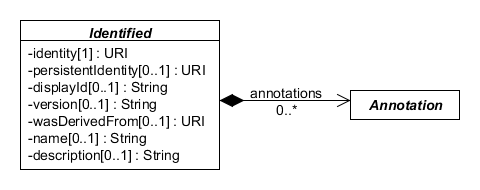
\includegraphics[scale=0.6]{uml/identified}
\caption[]{The Identified abstract class}
\label{uml:identified}
\end{center}
\end{figure}

All SBOL-defined classes are directly or indirectly derived from the \sbol{Identified}  class. This inheritance means that all SBOL objects are identified using \external{URI}s that uniquely refer to these objects within an SBOL document or at locations on the World Wide Web. As shown in \ref{uml:identified}, the \sbol{Identified} class includes the following properties: \sbol{identity}, \sbol{persistentIdentity},  \sbol{version}, and \sbol{annotations}. The latter property is described separately in \ref{sec:annotations}.

\subsubsection*{The \sbolheading{identity} property}
\label{sec:identity}
The \sbol{identity} property is required by all \sbol{Identified} objects and has a data type of \external{URI}. This \external{URI} serves to uniquely identify an SBOL object. Although most SBOL properties are defined by SBOL and serialized with its namespace, the \sbol{identity} property is defined by the analogous RDF \external{about} property and is serialized with the RDF namespace as follows:

\external{http://www.w3.org/1999/02/22-rdf-syntax-ns\#about}.

This substitution is in keeping with the commitment of the SBOL community to the practical reuse of existing standards.

\subsubsection*{The \sbolheading{persistentIdentity} property}
\label{sec:persistentIdentity}
The \sbol{persistentIdentity} property is optional and also has a data type of \external{URI}. This \external{URI} serves to uniquely refer to a set of SBOL objects that are different versions of each other. An SBOL object can referred to by either its \sbol{identity} \external{URI} or its \sbol{persistentIdentity} \external{URI}. In the latter case, this reference only holds if the SBOL object has the latest \sbol{version} property out of those objects with the same \sbol{persistentIdentity}.

\subsubsection*{The \sbolheading{displayId} property}
\label{sec:displayId}
An optional identifier, with a data type of \external{String}. It is intended to be an intermediate between \sbol{name} and \sbol{identity}: machine-friendly text that is not necessarily unique, and more human-friendly than the full URI of an \sbol{identity}.

\Ctodo{This is the wrong syntax.  It allows "-" and "." which we do not allow.}

In particular, displayId string MUST be compliant with type \external{http://www.w3.org/TR/xmlschema-2/\#NCName}

\subsubsection*{The \sbolheading{version} property}
\label{sec:version}

\Ctodo{need to somehow explain stuff about Maven versioning}
The \sbol{version} property is optional and has a data type of \external{String}. This property can be used to compare two SBOL objects with the same \sbol{persistentIdentity}.

\subsection {Documented}
\label{sec:Documented}
The Documented class in SBOL represents objects that can be decorated with human-readable properties, such as name and description. This class extends \sbol{Identified} with three additional data properties: \sbol{displayId}, \sbol{name}, and \sbol{description} (\ref{uml:documented}). 

\begin{figure}[ht]
\begin{center}
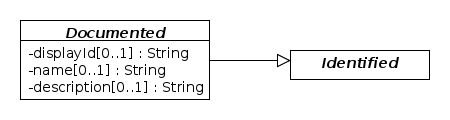
\includegraphics[scale=0.6]{uml/documented}
\caption[]{The Documented class}
\label{uml:documented}
\end{center}
\end{figure}

\subsubsection*{The \sbolheading{name} property}
\label{sec:name}
An optional, human readable name property, with a data type of \external{String}. It is intended to be displayed to a human when visualising SBOL objects.  
If a \sbol{Documented} object lacks a name, it is expected that software tools will instead display the entity's \sbol{displayId} or \sbol{identity} as a last resort.

\Ctodo{name is no longer the preferred, also we need to say that displayId should be to the best of one's ability locally unique.  And RECOMMEND that any software tool give people the ability to switch perspectives between looking at names (for human-friendliness) and looking at displayIds (for better uniqueness).}

\Ctodo{Need to require use of DublinCore names and show examples of them: non-stanard mappings per Matt: Title vs. Name, descripton is dcterms:description}

\Ctodo{SHOULD sanitize your displayId entries}
\Ctodo{need to add sanitization to libSBOLj}

\subsubsection*{The \sbolheading{description} property}
\label{sec:description}
An OPTIONAL, free text property with the data type of \external{String}, intended to contain a more thorough description of an object.


\subsection {TopLevel}
\label{sec:TopLevel}
\sbol{TopLevel} is an abstract class that is extended by any \sbol{Documented} object that can be found at the top level of a SBOL file, i.e., any SBOL object that is not nested inside another object when written to a file. Instead of nesting, composite \sbol{TopLevel} objects link to their subordinate \sbol{TopLevel} objects via \external{URI}s when written to a file. For example, a composite \sbol{Component} object A would link to its sub-Component object B using B's \external{URI}. The TopLevel classes defined by this specification are \sbol{Sequence}, \sbol{ComponentDefinition}, \sbol{ModuleDefinition}, \sbol{Module}, \sbol{Collection} and \sbol{GenericTopLevel} (\ref{uml:toplevel}).

\begin{figure}[ht]
\begin{center}
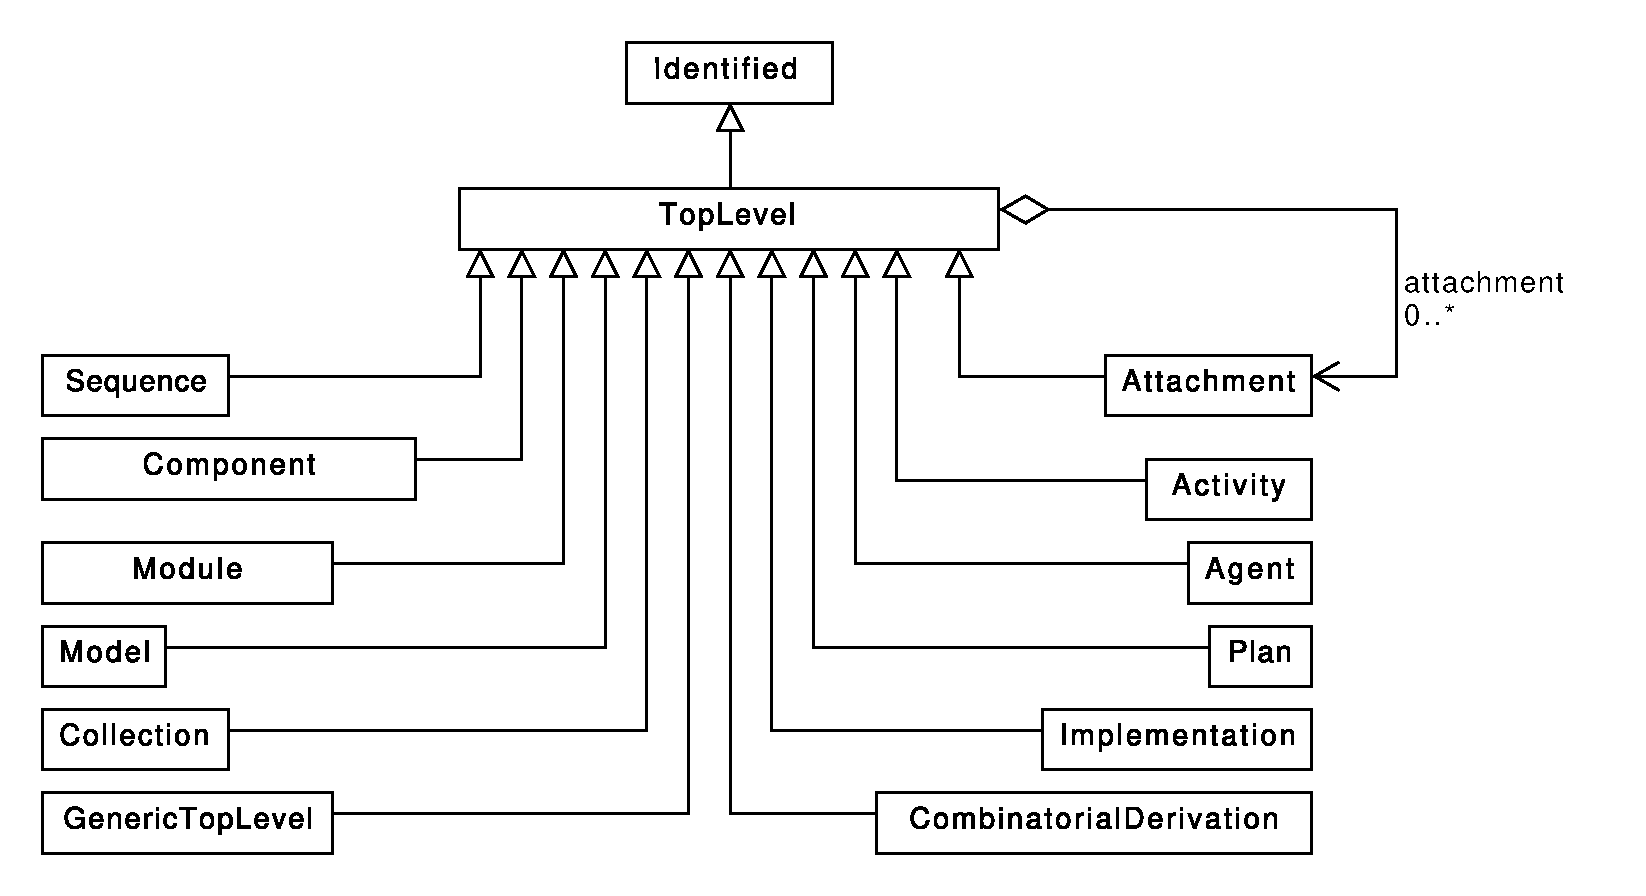
\includegraphics[width=\textwidth]{uml/toplevel}
\caption[]{The TopLevel classes}
\label{uml:toplevel}
\end{center}
\end{figure}

\Ctodo{Make the left-right order in this figure match the order of the following sections}



\subsection{Sequence}
\label{sec:Sequence}
The \sbol{Sequence} class is used to encode the primary structure of a \sbol{ComponentDefinition} object and the encoding used to capture this information.

\begin{figure}[ht]
\begin{center}
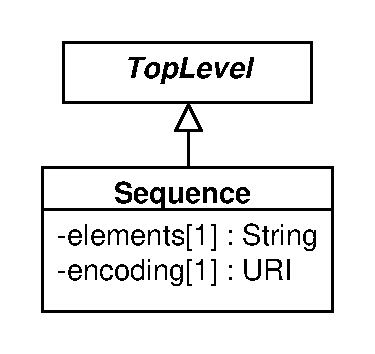
\includegraphics[scale=0.6]{uml/sequence}
\caption[]{Sequence class}
\label{uml:sequence}
\end{center}
\end{figure}


\subsubsection*{The \sbolheading{elements} property}
\label{sec:elements}
A REQUIRED \external{String} of characters that represent the constituents of biological molecule, for example   nucleic acid symbols for DNA molecules. 

\Ctodo{give non-DNA example too -JSB}

\subsubsection*{The \sbolheading{encoding} property}
\label{sec:encoding}
Required. \sbol{Sequence} objects identify their type of encoding with a \external{URI}. For example, a \sbol{Sequence} object that encodes a DNA sequence would have an \external{IUPAC DNA} encoding, while a \sbol{Sequence} object that encodes the chemical structure of glucose might have a \external{simplified molecular-input line-entry system (SMILES)} encoding (\ref{tbl:sequence_encodings}).

\Ctodo{These are RECOMMENDED.}

%A Summary of letters for nucleic acids and aminoacids
\begin{table}[ht]
  \begin{edtable}{tabular}{ll}
    \toprule
    \textbf{ComponentDefinition Type} & \textbf{Encoding} \\
    \midrule
    DnaRegion,RnaRegion  & \url{http://www.chem.qmul.ac.uk/iubmb/misc/naseq.html}\\
    Protein		 & \url{http://www.chem.qmul.ac.uk/iupac/AminoAcid/}\\
    SmallMolecule    & \url{http://www.opensmiles.org/opensmiles.html}\\
    \bottomrule
  \end{edtable}
  \caption{URIs for the encoding property and the corresponding ComponentDefiniton types, which are BioPAX terms.}
  \label{tbl:sequence_encodings}
\end{table}
\Ctodo{Need to fix the caption of table 1, and need to match the biopa terms and give a forward pointer to table 2}
\Ctodo{Matthew Pocock is in charge of deciding whether any more ontologies should be listed.}
\Ctodo{GM: Add the BioPax terms Dna and Rna in addition to DnaRegion and RnaRegion.}


The serialization of \sbol{Sequence} objects has the following form:
\lstsetsbol
\begin{lstlisting}
<sbol:Sequence rdf:about="...">
      ...
  [\emph{one}] <sbol:elements>...</sbol:elements> [\emph{element}]
  [\emph{one}] <sbol:encoding rdf:resource="..."/> [\emph{element}]
</sbol:Sequence>
\end{lstlisting}

The example below shows the serialization of a \sbol{Sequence} object for a promoter. Nucleotide sequences are represented with the \sbol{elements} property and the \sbol{encoding} is serialized as a URI value. 

\lstsetsbol
\begin{lstlisting}
<sbol:Sequence rdf:about="http://www.partsregistry.org/Part:BBa_J23119:Design">
  <sbol:elements>ttgacagctagctcagtcctaggtataatgctagc</sbol:elements>
  <sbol:encoding rdf:resource="http://www.chem.qmul.ac.uk/iubmb/misc/naseq.html"/>
</sbol:Sequence>
\end{lstlisting}


\subsection{ComponentDefinition}
\label{sec:ComponentDefinition}

A \sbol{ComponentDefinition} is an entity in the biological system that is being represented. Its motivating usage is to represent objects with designed sequences (DNA, RNA, or proteins), but it can also represent any other object that is part of or interacts with a design, such as small molecules, molecular complexes, or light.
(this is a generalization from prior versions of SBOL, which only represented DNA).

% Figure has some classes named incorrectly
\begin{figure}[ht]
\begin{center}
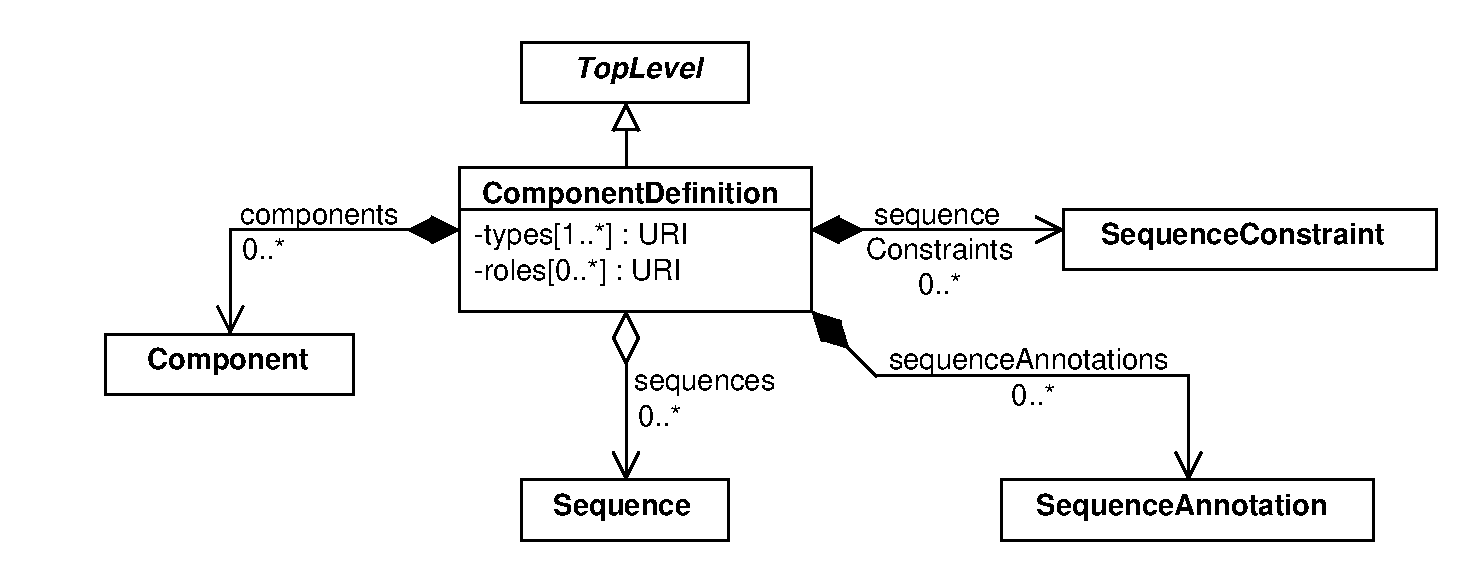
\includegraphics[width=0.95\textwidth]{uml/component_definition}
\caption[]{ComponentDefinition}
\label{uml:component_definition}
\end{center}
\end{figure}



\LDtodo{Examples of ontologies for non-molecular type gs (eg, light)...?}
\subsubsection*{The \sbolheading{types} property}
\label{sec:types}
Every \sbol{ComponentDefinition} MUST have at least one \sbol{types} \external{URI} that identifies a term from an appropriate ontology, such as the BioPAX ontology (some recommended examples are given in \ref{tbl:componentdefinition_types}) or the ontology of Chemical Entities of Biological Interest (ChEBI). A type URI documents the category of biochemical or physical entity (for example DNA, protein, or RNA) that a \sbol{ComponentDefinition} object abstracts for the purpose of engineering design. If a \sbol{ComponentDefinition} object has multiple type URIs, then they MUST identify synonymous terms.

\Ctodo{It is REQUIRED that if your component fits a Table 2 term, that you MUST use that term as at least one of the terms.}

\begin{table}[ht]
  \begin{edtable}{tabular}{ll}
    \toprule
    \textbf{Entity Type} & \textbf{BioPAX Term} \\
    \midrule
    DNA  & \url{http://www.biopax.org/release/biopax-level3.owl#DnaRegion}\\
    RNA  & \url{http://www.biopax.org/release/biopax-level3.owl#RnaRegion}\\
    Protein  & \url{http://www.biopax.org/release/biopax-level3.owl#Protein}\\
    Small Molecule  & \url{http://www.biopax.org/release/biopax-level3.owl#SmallMolecule}\\  
    \bottomrule
  \end{edtable}
  \caption{BioPAX terms to specify the types of ComponentDefinition objects.}
  \label{tbl:componentdefinition_types}
\end{table}

\subsubsection*{The \sbolheading{roles} property}
\label{sec:roles}

The \sbol{roles} of a ComponentDefinition object MUST contain at least one URI.  These identify ontology terms that clarify a \sbol{ComponentDefinition} object's potential function in a biological context. For example, a \sbol{ComponentDefinition} for a DNA component might have a role of ``promoter'' or ``terminator,'' terms taken from the Sequence Ontology (SO). A ComponentDefinition object for a protein, on the other hand, might have a role of ``transcription factor'' or ``protease.'' 
\LDtodo{Taken from what ontology?}

The \sbol{roles} are analogous to the \external{type} of a \external{DnaComponent} object in SBOL Version 1.1. 


\subsubsection*{The \sbolheading{components} property}
\label{sec:components}

If \sbol{ComponentDefinition} class is analogous to a blueprint or parts specification sheet for a biological part. In contrast, the \sbol{Component} class represents specific occurrences of parts within a design.  This allows biological designs that use a component more than once.
The \sbol{components} property specifies a collection of such parts contained within a particular \sbol{ComponentDefinition}.


\subsubsection*{The \sbolheading{sequence} property}
\label{sec:sequence}
The sequence property is optional and includes the URI for a corresponding \sbol{Sequence} object.

\subsubsection*{The \sbolheading{sequenceConstraint} property}
\label{sec:sequenceConstraint}

\Ctodo{This needs to be explained}

\subsubsection*{The \sbolheading{sequenceAnnotation} property}
\label{sec:sequenceAnnotation}

\Ctodo{This needs to be better explained. -JSB}

A \sbol{ComponentDefinition} object can define its structure by linking to objects that belong to the Component, Sequence, SequenceAnnotation, and SequenceConstraint classes. These classes are described below.

\subsubsection*{Serialization}
The parents of the \sbol{ComponentDefinition} class are \sbol{TopLevel} and, transitively, \sbol{Documented} and \sbol{Identified}. As a result, inherited properties are serialised as explained for these parent classes. The sequence property of a \sbol{ComponentDefinition} object includes a URI to a \sbol{Sequence} object and this URI is serialized as an \external{rdf:resource}. The \sbol{types} property may include a collection of type URIs and is serialized as an implicit collection, ignoring the property name ``types''. The \sbol{roles} property is also similarly serialized as an implicit collection of sbol:roles properties.

\Ctodo{Add the serialization descriptions to parent classes; make sure everything has its serialization}
\lstsetsbol
\begin{lstlisting}
<sbol:ComponentDefinition rdf:about="...">
               ...
  [\emph{zero or one}]  <dcterms:title>...</dcterms:title> [\emph{element}]
  [\emph{zero or one}]  <dcterms:description>...</dcterms:description> [\emph{element}]
  [\emph{zero or one}]  <sbol:sequence rdf:resource="..."/> [\emph{element}]
  [\emph{one or more}]  <sbol:type rdf:resource="..."/> [\emph{elements}]
  [\emph{one or more}]  <sbol:role rdf:resource="..."/> [\emph{elements}]    
  [\emph{zero or more}] <sbol:subComponent>
                 <sbol:Component rdf:about="...">...</sbol:Component>
               </sbol:subComponent> [\emph{elements}]
  [\emph{zero or more}] <sbol:sequenceAnnotation>
                 <sbol:SequenceAnnotation rdf:about="...">...</sbol:SequenceAnnotation>
               </sbol:sequenceAnnotation> [\emph{elements}]        
  </sbol:ComponentDefinition>
\end{lstlisting}
\Ctodo{We need to have an explanation of how to interpret these, and also have a pointer to it from each example.}

The example below shows the serialization of a simple \sbol{ComponentDefinition} object. The \external{DnaRegion} from BioPAX and \external{CHEBI:4705} from CHEBI are used to indicate the type of the biological entity as a DNA molecule. Its role is specified via the generic \external{SO:0000167} (\external{promoter}) and more specific \external{SO:0000613} (\external{bacterial\_RNApol\_promoter}) terms.

\lstsetsbol
\begin{lstlisting}
<sbol:ComponentDefinition rdf:about="http://www.partsregistry.org/Part:BBa_J23119">
  <dcterms:title>J23119 promoter</dcterms:title>
  <dcterms:description>Constitutive promoter</dcterms:description>
  <sbol:type rdf:resource="http://identifiers.org/chebi/CHEBI:4705"/>
  <sbol:type rdf:resource="http://www.biopax.org/release/biopax-level3.owl#DnaRegion"/>
  <sbol:role rdf:resource="http://identifiers.org/so/SO:0000167"/>
  <sbol:role rdf:resource="http://identifiers.org/so/SO:0000613"/>
  <sbol:sequence rdf:resource="http://www.partsregistry.org/Part:BBa_J23119:Design"/>
</sbol:ComponentDefinition>
\end{lstlisting}


\subsubsection{ComponentInstance}
\label{sec:ComponentInstance}

\begin{figure}[ht]
\begin{center}
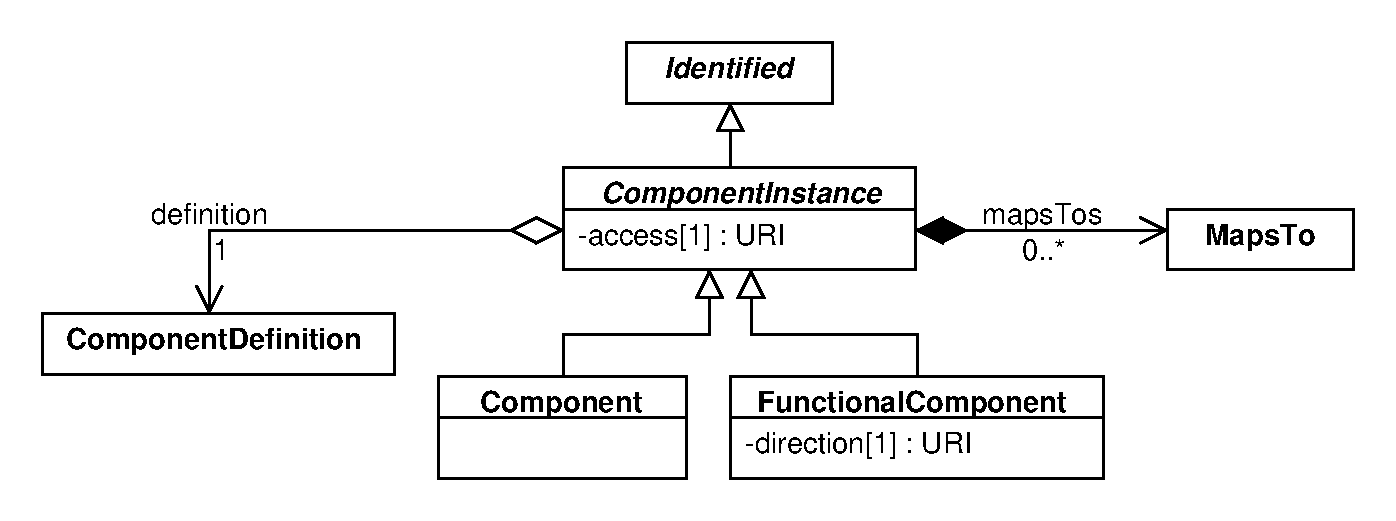
\includegraphics[scale=0.6]{uml/component_instance}
\caption[]{ComponentInstance}
\label{uml:component}
\end{center}
\end{figure}

When a \sbol{ComponentDefinition} is used as an element of a larger design, each separate use is represented by a \sbol{ComponentInstance} object.  
The \sbol{ComponentInstance} class is abstract, so every usage must be as one of its two subclasses:
\begin{itemize}
\item \sbol{Component} is used for specifying hierarchical structure, and can be linked to by the properties of parts of a \sbol{ComponentDefinition}.
\item \sbol{FunctionalComponent} is used for describing function in a \sbol{Module}, and can be linked to by the properties of parts of a \sbol{Module}.  It is described in the \sbol{Module} section.
\end{itemize}

\paragraph{The \sbolheading{componentDefinition} property}
\label{sec:componentDefinition}

Every \sbol{ComponentInstance} MUST be associated with precisely one
\sbol{ComponentDefinition}, which is the design that it is an instance of.

\paragraph{The \sbolheading{mapsTo} property}
\label{sec:mapsTo}

\Ctodo{Need to make sure all MapsTo statements are correct}
The \sbol{mapsTo} property links \sbol{Component} objects (both Components and FunctionalComponents) together within a larger design, indicating that they refer to the same entity.

The third data field, ``mappings'', is a set of MapsTo objects that link between other ComponentInstance objects at the same level of the design hierarchy as well as other ComponentInstance objects that are lower in the design hierarchy, thereby composing these objects with greater specificity (see first module example).

\paragraph{The \sbolheading{access} property}
\label{sec:access}

The \sbol{access} determines whether a \sbol{ComponentInstance} 
can be identified with a part in a larger design via \sbol{MapsTo}.
The \sbol{access} property must be set to one of the following URIs:

\begin{itemize}
\item \url{http://sbols.org/v2#public}
  If the access is public, the \sbol{ComponentInstance} MAY be linked to by \sbol{MapsTo} objects.

\item \url{http://sbols.org/v2#private}
  If the access is private, the \sbol{ComponentInstance} MUST NOT be linked by any \sbol{MapsTo} object.
\end{itemize}


\subsubsection{Component}
\label{sec:Component}
Composition of the structural layer of SBOL designs is accomplished using \sbol{Component} objects. Each \sbol{Component} instance is part of a \sbol{ComponentDefinition} object, associated with it by the \sbol{components} property to represent  physical composition.  

All \sbol{Component} objects directly referenced within a \sbol{ComponentDefinition}'s \sbol{SequenceAnnotation} or \sbol{SequenceConstraint} parts MUST be associated with that \sbol{ComponentDefinition} by means of its \sbol{components} property.


\subsubsection{SequenceAnnotation}
\label{sec:SequenceAnnotation}
The \sbol{SequenceAnnotation} class describes a precisely known location of interest on the \sbol{Sequence} object linked by its parent \sbol{ComponentDefinition} object.  It can also optionally associate this location with a \sbol{Component} object. \sbol{SequenceAnnotation} objects specify their location using a \sbol{Location} object, as described below.

\Dtodo{Can we change location to locations (1..*) and eliminate MultiRange class?}

\begin{figure}[ht]
\begin{center}
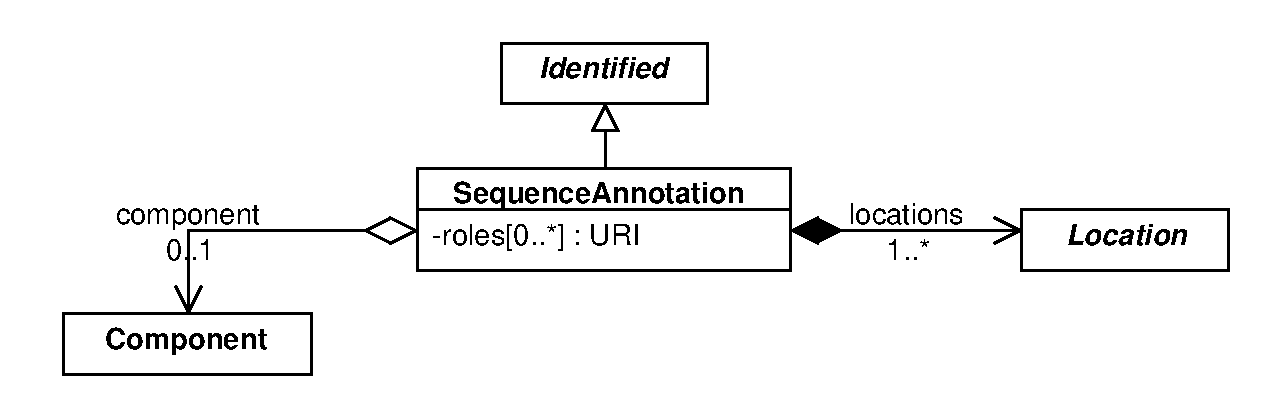
\includegraphics[scale=0.6]{uml/sequence_annotation}
\caption[]{SequenceAnnotation class}
\label{uml:sequence_annotation}
\end{center}
\end{figure}

\paragraph{The \sbolheading{location} property}
Every \sbol{SequenceAnnotation} MUST have a location property. The value of this property is a nested \sbol{Location} object.

\paragraph{The \sbolheading{component} property}
\sbol{SequenceAnnotation} objects MAY use this property to link location information to a \sbol{Component} object, by specifying its URI.

\Ctodo{Separate serialization better - give paragraph/subsubsec headers}

The serialization of SequenceAnnotation objects MUST be carried out according to the template below. In this template, A\_LOCATION\_SUBCLASS represents one of the Location subclasses.
\lstsetsbol
\begin{lstlisting}
<sbol:SequenceAnnotation rdf:about="...">
               ...   
  [\emph{zero or one}] <sbol:component rdf:resource="..."/> [\emph{element}] 
  [\emph{one}]         <sbol:location>
                 <sbol:A_LOCATION_SUBCLASS rdf:about="...">...</sbol:A_LOCATION_SUBCLASS>
               </sbol:location> [\emph{element}] 
</sbol:SequenceAnnotation>
\end{lstlisting}

\Ctodo{Make sure it's clear these templates specify content, not order}



\subsubsection{Location}
\label{sec:Location}
The Location class is extended by the \sbol{Range}, \sbol{MultiRange}, \sbol{Cut}, and \sbol{GenericLocation} classes.


\begin{figure}[ht]
\begin{center}
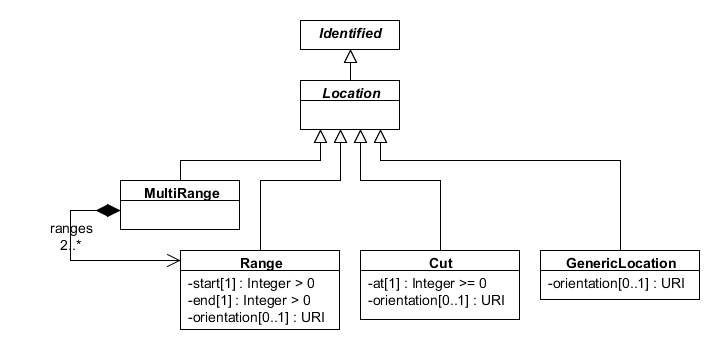
\includegraphics[scale=0.6]{uml/location}
\caption[]{Location class}
\label{uml:location}
\end{center}
\end{figure}




\paragraph{Range}
\label{sec:Range}
A \sbol{Range} object specifies inclusive start and end positions. These properties are required in \sbol{Range} objects and they can have \external{integer} values greater than zero. A \sbol{Range} object also includes an  ``orientation'' property, for example to to specify directionality on a potentially double-stranded \sbol{Component} object.

\subparagraph{The \sbolheading{start} property}
Specifies the start of a \sbol{Range}. This property is REQUIRED and can have \external{integer} values greater than zero.

\subparagraph{The \sbolheading{end} property}
Specifies the end of a \sbol{Range}. This property is REQUIRED and can have \external{integer} values greater than zero.

\subparagraph{The \sbolheading{orientation} property}
\label{sec:orientation}
This OPTIONAL property has a URI value. For \sbol{ComponentDefinition} objects representing DNA molecules, it is RECOMMENDED to use one of the values in \ref{tbl:orientation_types}. 

\begin{table}[ht]
  \begin{edtable}{tabular}{l}
    \toprule
    \textbf{Orientation Types}  \\
    \midrule
    http://sbols.org/v2\#inline\\
    http://sbols.org/v2\#reverseComplement\\
    \bottomrule
  \end{edtable}
  \caption{URI constants for orientation values}
  \label{tbl:orientation_types}
\end{table}

The serialization of Range objects has the following form:
\lstsetsbol
\begin{lstlisting}
<sbol:Range rdf:about="...">
               ...   
  [\emph{one}]         <sbol:start>...</sbol:start> [\emph{element}] 
  [\emph{one}]         <sbol:end>...</sbol:end> [\emph{element}] 
  [\emph{zero or one}] <sbol:orientation rdf:resource="..."/> [\emph{element}] 
</sbol:Range>
\end{lstlisting}

The example below shows the serialization of a \sbol{Range} object. It specifies the region between 56 and 68, and the orientation is given as \external{inline}.
\lstsetsbol
\begin{lstlisting}
<sbol:Range rdf:about="http://www.partsregistry.org/Part:BBa_F2620/anno2/range">
  <sbol:orientation rdf:resource="http://sbols.org/v2#inline"/>
  <sbol:start>56</sbol:start>
  <sbol:end>68</sbol:end>
</sbol:Range>
\end{lstlisting}

\paragraph{MultiRange}
\label{sec:MultiRange}
A \sbol{MultiRange} object represents a location that is specified by multiple \sbol{Range} objects. For example, this capability can be used to specify a \sbol{ComponentDefinition} object that represents the introns or exons of a eukaryotic gene.

\paragraph{Cut}
\label{sec:Cut}
The \sbol{Cut} class has been introduced to enable the specification of a location between two indices. 
Each \sbol{Cut} object has properties, \sbol{at} and \sbol{orientation}.

\subparagraph{The \sbolheading{at} property}
\label{sec:at}
The REQUIRED \sbol{at} property is an index greater than or equal to zero that specifies the index just before the location represented by the Cut object. 
A Cut object with \sbol{at} equal to zero represents the location just before index one (even though there is no zero index on Structure objects in SBOL). 

\subparagraph{The \sbolheading{orientation} property}
This OPTIONAL property has a URI value. For \sbol{ComponentDefinition} objects representing DNA molecules, it is RECOMMENDED to use one of the values in \ref{tbl:orientation_types} (above with \sbol{Range}).


\paragraph{GenericLocation}
\label{sec:GenericLocation}

While the \sbol{Range} and \sbol{Cut} classes are best suited to
describing locations on sequential structures, the
\sbol{GenericLocation} is included as a hook for extensions, e.g., for
describing locations in non-sequential structures.

\Ctodo{Need serialization examples for MultiRange, Cut, and GenericLocation}
\Ctodo{Make sure that every property has a section label so that it hyperlinks correctly}

\subsubsection{SequenceConstraint}
\label{sec:SequenceConstraint}
A \sbol{ComponentDefinition} object can link to \sbol{SequenceConstraint} objects to assert various kinds of structural restrictions between two \sbol{Component} objects that are its subcomponents. 
The purpose of \sbol{SequenceConstraint} is to allow partial designs to be specified when the precise identity, location, or ordering of \sbol{Component} objects is not yet fully determined.

A \sbol{SequenceConstraint} object requires \sbol{restriction}, \sbol{subject} and \sbol{object} properties to specify such constraints.

\Dtodo{Should SequenceConstraint be Documented?}

\begin{figure}[ht]
\begin{center}
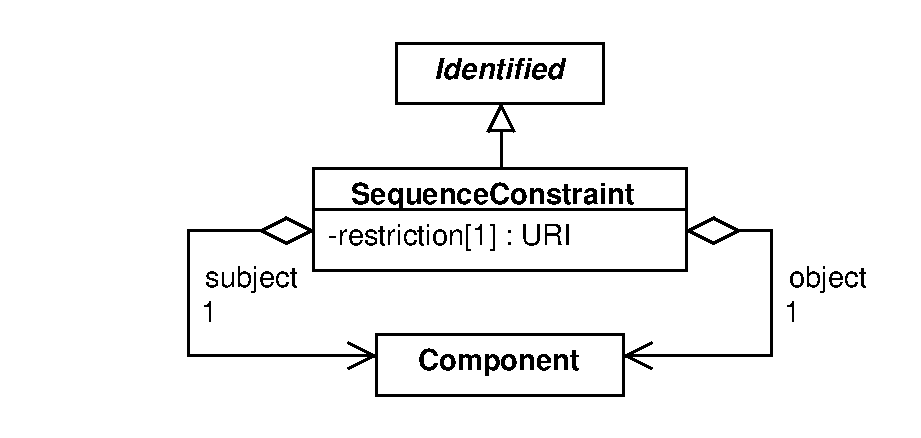
\includegraphics[scale=0.6]{uml/sequence_constraint}
\caption[]{SequenceConstraint class}
\label{uml:sequence_constraint}
\end{center}
\end{figure}

\paragraph{The \sbolheading{subject} property}
\label{sec:subject}
This REQUIRED property specifies the \sbol{identity} URI of the first \sbol{Component} object in the relation.

\Ctodo{Need to document that you can reference a persistentIdentity or an identity when you reference a version.  Everywhere we say ``URI'' for an SBOL object, it means one of these two properties}

\Ctodo{Remove ``identity'' for names of URIs everywhere}

\paragraph{The \sbolheading{object} property}
\label{sec:object}
This REQUIRED property specifies the URI \sbol{identity} of the second \sbol{Component} object in the relation.

\paragraph{The \sbolheading{restriction} property}
\label{sec:restriction}

This REQUIRED property specifies a URI that identifies the type of relationship between the \sbol{subject} and \sbol{object} \sbol{Component} objects. 
The RECOMMENDED values for this property are given in \ref{tbl:restriction_types}.

Note: With regards to SBOL Version 1.1., this is a generalization of former \sbol{SequenceAnnotation} property \external{precedes}.

\begin{table}[ht]
  \begin{edtable}{tabular}{ll}
    \toprule
    \textbf{Restriction Types} & Subject/Object Relation \\
    \midrule
    http://sbols.org/v2\#precedes & Subject location is strictly less than object location \\
    http://sbols.org/v2\#sameOrientationAs & Subject and object have equal orientation URIs\\
    http://sbols.org/v2\#oppositeOrientationAs & Object orientation is ``opposite'' of subject\\    
    \bottomrule
  \end{edtable}
  \caption{URI constants for restriction values}
  \label{tbl:restriction_types}
\end{table}

\Ctodo{We need things like nextTo and overlapping, and think we might be able to get it from region-connection-calculus ontology}

\paragraph{Serialization}

The serialization of \sbol{SequenceConstraint} objects has the following form:
\lstsetsbol
\begin{lstlisting}
<sbol:SequenceConstraint rdf:about="...">
      ...
  [\emph{one}] <sbol:restriction rdf:resource="..."/> [\emph{element}]
  [\emph{one}] <sbol:subject rdf:resource="..."/> [\emph{element}]
  [\emph{one}] <sbol:object rdf:resource="..."/> [\emph{element}]
</sbol:SequenceConstraint>
\end{lstlisting}

The example below shows the serialization of a \sbol{SequenceConstraint} object. In the example, the constraint is included as part of a \sbol{ComponentDefinition} for a LacI repressible composite promoter and has a precedes restriction. This restriction states that the subject \sbol{Component} for the core promoter precedes the object \sbol{Component} for the LacI operator in the composite promoter definition. Such restriction is especially useful to specify incomplete designs and the final design may include other components between the subject and object components. 
\lstsetsbol
\begin{lstlisting}
<sbol:SequenceConstraint rdf:about="http://www.partsregistry.org/Part:BBa_K174004/r1">
  <sbol:subject rdf:resource="http://www.partsregistry.org/Part:BBa_K174004#pspac"/>
  <sbol:object rdf:resource="http://www.partsregistry.org/Part:BBa_K174004#LacIoperator"/>
  <sbol:restriction rdf:resource="http://sbols.org/v2#precedes"/>
</sbol:SequenceConstraint>
\end{lstlisting}

\Ctodo{In every serialization example, make sure something differs in order from the template, to more intuitively illustrate the unimportance of order --> actually no, jake shoud put bac the examples he messed with}

\subsection{Model}
\label{sec:Model}

\begin{figure}[ht]
\begin{center}
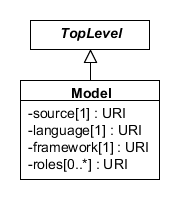
\includegraphics[scale=0.6]{uml/model}
\caption[]{}
\label{uml:model}
\end{center}
\end{figure}

SBOL's \sbol{Model} objects are placeholders that point to some external modeling mechanism, with some additional meta-data to enable better reasoning about the contents of that external mechanism.
In this way, there is minimal duplication of standardization efforts and users of SBOL can specify the quantitative function of \sbol{ModuleDefinition} objects in a well-developed language of their choice. 

Each \sbol{Model} object specifies the location of the actual content of a qualitative/quantitative model, the language the model is implemented with, the modelling framework and the model's role(s). 

\subsubsection*{ The \sbolheading{source} property}
This REQUIRED property is a URI that specifies the actual location of a qualitative or quantitative model.

\subsubsection*{ The \sbolheading{language} property}
This REQUIRED property is a URI that specifies the language the model is implemented with. 
Values for this URI are RECOMMENDED to be chosen from the EMBRACE Data and Methods (EDAM) ontology where possible. A few suggested model types and corresponding URI values are shown in \ref{tbl:model_types}.

\LDtodo{Make sure EDAM goes in ontology best-practices section}

\begin{table}[ht]
  \begin{edtable}{tabular}{ll}
    \toprule
    \textbf{Model Language} & \textbf{URI} \\
    \midrule
    SBML  & \url{http://identifiers.org/edam/format_2585}\\
    CellML		 & \url{http://identifiers.org/edam/format_3240}\\
    BioPAX    & \url{http://identifiers.org/edam/format_3156}\\
    \bottomrule
  \end{edtable}
  \caption{Commonly used model languages and their corresponding URIs.}
  \label{tbl:model_types}
\end{table}


\subsubsection*{ The \sbolheading{framework} property}
This REQUIRED property is a URI that specifies the modelling framework that a model is implemented within. 
Values for this URI are RECOMMENDED to be chosen from the SBO's modelling framework terms where possible. A few suggested model frameworks and corresponding URI values are shown in \ref{tbl:model_frameworks}.

\begin{table}[ht]
  \begin{edtable}{tabular}{ll}
    \toprule
    \textbf{Framework} & \textbf{URI} \\
    \midrule
    Continuous  & \url{http://identifiers.org/biomodels.sbo/SBO:0000062}\\
    Discrete & \url{http://identifiers.org/biomodels.sbo/SBO:0000063}\\
    \bottomrule
  \end{edtable}
  \caption{Example modelling frameworks and corresponding SBO terms.}
  \label{tbl:model_frameworks}
\end{table}

\LDtodo{Made sure SBO frameworks goes in ontology best-practices section}

\Ctodo{We are dropping the role property entirely --- make sure it gets deleted}

\subsubsection*{Serialization}

The serialization of \sbol{Model} objects has the following form:

\lstsetsbol
\begin{lstlisting}
<sbol:Model rdf:about="http://www.sbolstandard.org/examples/toogleswicth">
  ...
  [\emph{one}]         <sbol:source rdf:resource="..."/> [\emph{element}]
  [\emph{one}]         <sbol:language rdf:resource="..."/> [\emph{element}]
  [\emph{one}]         <sbol:framework rdf:resource="..."/> [\emph{element}]
  [\emph{one or more}] <sbol:role rdf:resource="..."/> [\emph{element}]
</sbol:Model>
\end{lstlisting}

The example below shows the serialization of a \sbol{Model} object. The model object includes information about the models of a toggle switch. The model is implemented in SBML using a continuous modelling framework. The source property shows the physical location of the SBML model, in a model repository. 
\lstsetsbol
\begin{lstlisting}
<?xml version="1.0" ?>
<rdf:RDF xmlns:rdf="http://www.w3.org/1999/02/22-rdf-syntax-ns#" xmlns:sbol="http://sbols.org/v2#">
  <sbol:Model rdf:about="http://www.sbolstandard.org/examples/toogleswicth">
    <sbol:role rdf:resource="http://sbols.org/v2#module_model"/>
    <sbol:language rdf:resource="http://identifiers.org/edam/format_2585"/>
    <sbol:source rdf:resource="http://virtualparts.org/part/pIKE_Toggle_1"/>
    <sbol:framework rdf:resource="http://identifiers.org/biomodels.sbo/SBO:0000062"/>
  </sbol:Model>
</rdf:RDF>

\end{lstlisting}
\label{ser:Model}



\Ctodo{This section has not been edited much compared to other sections. We need to explain classes and their properties a bit more in detail.}
\subsection{ModuleDefinition}
\label{sec:ModuleDefinition}

\begin{figure}[ht]
\begin{center}
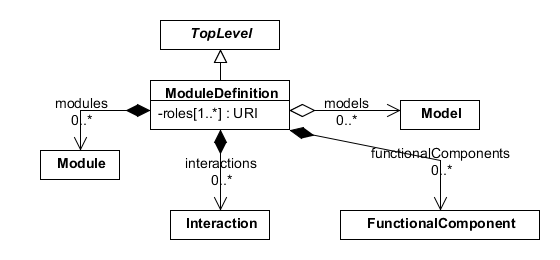
\includegraphics[scale=0.6]{uml/module_definition}
\caption[]{ModuleDefinition}
\label{uml:module_definition}
\end{center}
\end{figure}

The \sbol{ModuleDefinition} class is the hub where the structural and functional aspects of genetic designs come together to form a complete picture of the design. 
A \sbol{ModuleDefinition} object is composed from zero or more \sbol{FunctionalComponent}, \sbol{Module}, and \sbol{Interaction} objects, and links to zero or more \sbol{Model} objects. 
A \sbol{ModuleDefinition} object relies on the ``direction'' data fields of its \sbol{FunctionalComponent} objects to specify whether they serve as its inputs or outputs.
\Ctodo{the direction bit needs to be said much more clearly}

\subsubsection*{The \sbolheading{roles} property}
This property is OPTIONAL and may include a set of URIs that specifies the intended use of a \sbol{ModuleDefinition} entity. 
These URIs may identify terms for abstract module roles, such as``inverter'' or ``AND gate'', or they may identify terms for purely biological roles, such as ``metabolic pathway'' and ``signaling cascade''.
\Ctodo{make this sentence clearer}

\Ctodo{Make these more paralell to componentdefinition in the way that they are written}
\subsubsection*{The \sbolheading{models} property}
This property is OPTIONAL and includes identities of associated \sbol{Model} entities.

SBOL's \sbol{Model} objects are used to link genetic descriptions of biological parts and their interactions to computational models.
A ModuleDefinition object can link to more than one model since each one can encode different levels of functional detail and play different roles in engineering design. 
\Ctodo{clarify this bit with a bit more explanation and better content}

\Ctodo{make sure submodules --> modules}

\subsubsection*{The \sbolheading{modules} property}
This property is optional and includes a set of \sbol{Module} entities, which refer to \sbol{ModuleDefinition}s to be imported.
\Ctodo{use better language, like in componentdefinition}

\Ctodo{component --> functionalComponent in examples}
\subsubsection*{The \sbolheading{functionalComponents} property}
This property is optional and includes a set of \sbol{FunctionalComponent} entities. These entities are then used to describe biological interactions via \sbol{Participation} entities.

\Ctodo{use better language}

\subsubsection*{The \sbolheading{interactions} property}
This property is optional and includes a set of \sbol{Interaction} entities, which include \sbol{Participation} entities.

\subsubsection*{Serialization}

The serialization of \sbol{ModuleDefinition}s has the following form:
\lstsetsbol
\begin{lstlisting}
<sbol:ModuleDefinition rdf:about="...">
               ...
  [\emph{zero or one}]   <dcterms:title>...</dcterms:title> [\emph{element}]
  [\emph{zero or one}]   <dcterms:description>...</dcterms:description> [\emph{element}]
  [\emph{zero or more}]  <sbol:role rdf:resource="..."/> [\emph{elements}]
  [\emph{zero or more}]  <sbol:model rdf:resource="..."/> [\emph{elements}]
  [\emph{zero or more}] <sbol:component>
                 <sbol:FunctionalComponent rdf:about="...">...</sbol:FunctionalComponent >
               </sbol:component> [\emph{elements}]
  [\emph{zero or more}] <sbol:subModule>
                 <sbol:Module rdf:about="...">...</sbol:Module>
               </sbol:subModule> [\emph{elements}]
  [\emph{zero or more}] <sbol:interaction>
                 <sbol:Interaction rdf:about="...">...</sbol:Interaction>
               </sbol:interaction> [\emph{elements}]
</sbol:ModuleDefinition>
\end{lstlisting}

\Ctodo{Add an example, like for all the rest}


\subsubsection{FunctionalComponent}
\label{sec:FunctionalComponent}
Composition of the functional layer of SBOL designs is accomplished using \sbol{FunctionalComponent} objects. Each FunctionalComponent object is owned by a \sbol{ModuleDefinition} and serves as an explicit usage of a \sbol{Component} object for the purpose of fulfilling some function. In addition, each \sbol{FunctionalComponent} must specify via the ``direction'' field (\ref{tbl:functionalcomponent_directions}) whether it serves as an  input, output, both, or neither for its parent \sbol{ModuleDefinition} object. 
\Ctodo{Previously said a Module could own a FunctionalComponet, which i'm pretty sure is false -JB  Yes, it's false, fix it}

\LDtodo{Need to explain direction better.}

\sbol{FunctionalComponent} derives from \sbol{ComponentInstance}, and therefore has the definition and access properties. 


\begin{table}[ht]
  \begin{edtable}{tabular}{ll}
    \toprule
    \textbf{Direction URI} & \textbf{Description} \\
    \midrule
    \url{http://sbols.org/v2#inout}  & To indicate a \sbol{FunctionalComponent} can be used as both input or output\\
    \url{http://sbols.org/v2#in}  & To indicate a \sbol{FunctionalComponent} can be used as input\\
    \url{http://sbols.org/v2#out}  & To indicate a \sbol{FunctionalComponent} can be used as output\\
    \url{http://sbols.org/v2#none}  & To indicate a \sbol{FunctionalComponent} is neither input nor output\\
    \bottomrule
  \end{edtable}
  \caption{URIs for the direction property.}
  \label{tbl:functionalcomponent_directions}
\end{table}

\paragraph{Serialization}

The serialization of \sbol{FunctionalComponent}s has the following form.
\lstsetsbol
\begin{lstlisting}
<sbol:FunctionalComponent rdf:about="...">
  [\emph{zero or one}] <sbol:definition rdf:resource="..."/> [\emph{element}]
  [\emph{one}]         <sbol:access rdf:resource="..."/> [\emph{element}]
  [\emph{one}]         <sbol:direction rdf:resource="..."/> [\emph{element}]
</sbol:FunctionalComponent>
\end{lstlisting}

In the example below, the functional component is defined as public input or output. The component refers to the \texttt{Part:BBa\_R0010} promoter from the Parts Registry.
\lstsetsbol
\begin{lstlisting}
<sbol:FunctionalComponent rdf:about="http://sbolstandard.org/example/laci_inverter/fc/Part:BBa_R0010">
  <sbol:definition rdf:resource="http://www.partsregistry.org/Part:BBa_R0010"/>
  <sbol:access rdf:resource="http://sbols.org/v2#public"/>
  <sbol:direction rdf:resource="http://sbols.org/v2#inout"/>
</sbol:FunctionalComponent>
\end{lstlisting}

\subsubsection{Module}
\label{sec:Module}

\begin{figure}[ht]
\begin{center}
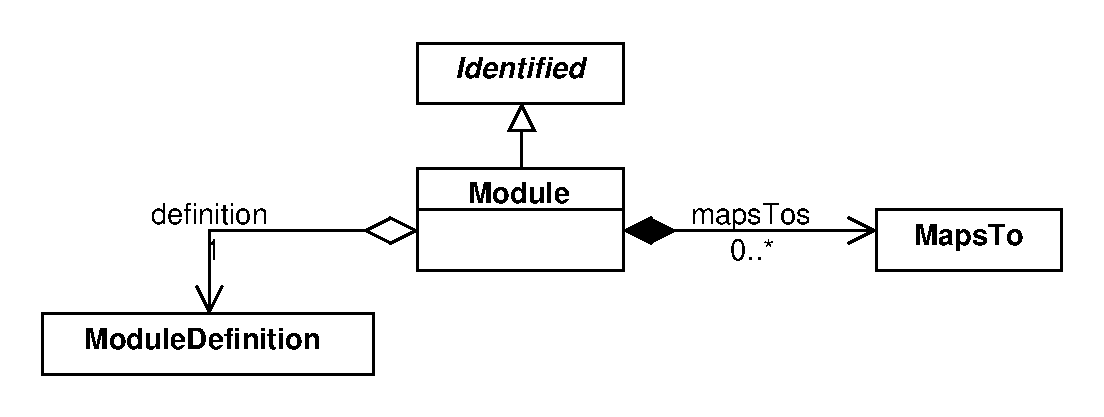
\includegraphics[scale=0.6]{uml/module}
\caption[]{Module}
\label{uml:module}
\end{center}
\end{figure}

The \sbol{Module} class enables the composition of \sbol{ModuleDefinition} objects from other, smaller \sbol{ModuleDefinition} objects. \textcolor{red}{The first data field, ``definition'', links to the ModuleDefinition object that is effectively a part of the Module object that owns the Module object.} The second data field, ``mappings'', is a set of MapsTo objects that link between the Component objects at the same level of the design hierarchy as the Module object and the Component objects that are lower in the design hierarchy, thereby composing these objects with greater specificity.

\Ctodo{mappings or mapsTo? --> mapsTo} 
\Ctodo{need to clean up this whole description}
\Ctodo{Is the notion of ``level of design hierarchy'' real?  I think it doesn't need to be stated here, it's actually a best practice. -->  it's a best practice.  Nick will write this better.}

The serialization of \sbol{Module}s has the following form.
\lstsetsbol
\begin{lstlisting}
<sbol:Module rdf:about="...">
  [\emph{one}]          <sbol:definition rdf:resource="..."/>[\emph{element}]
  [\emph{zero or more}] <sbol:mapping>
                 <sbol:MapsTo rdf:about="...">...</sbol:MapsTo>
               </sbol:mapping> [\emph{element}]
</sbol:Module>
\end{lstlisting}

\Ctodo{add an example}

\subsubsection{MapsTo}
\label{sec:MapsTo}

\begin{figure}[ht]
\begin{center}
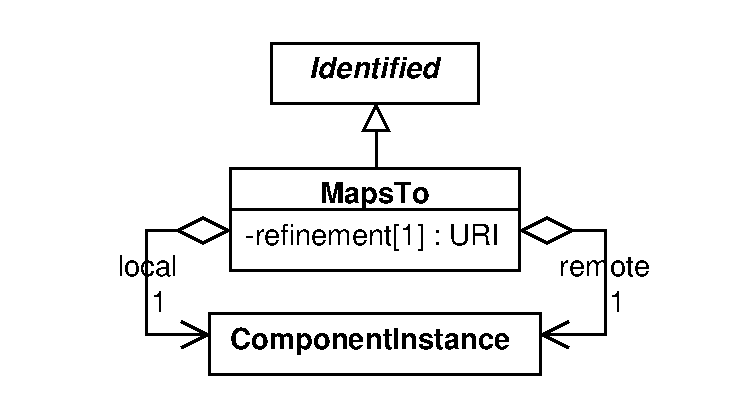
\includegraphics[scale=0.6]{uml/maps_to}
\caption[]{}
\label{uml:maps_to}
\end{center}
\end{figure}
The \sbol{MapsTo} class serves as a means of linking between \sbol{ComponentInstance} objects (both \sbol{Component}s and \sbol{FunctionalComponent}s) at different levels of the design hierarchy. For example, when a child \sbol{ModuleDefinition} object is instantiated inside a parent \sbol{ModuleDefinition} object, a \sbol{MapsTo} object is used to link these two ModuleDefinitions. MapsTo has properties to specify components from the parent and child entities, and also to specify how these components are linked.

\Ctodo{need to explain the whole 3-way mapsto model and importation better}

\paragraph{The local property}
This required property is used to specify the \sbol{ComponentInstance} from the parent entity.

\paragraph{The remote property}
This required property is used to specify the \sbol{ComponentInstance} from the child entity being imported by the parent.

\paragraph{The refinement property}
Each \sbol{MapsTo} entity must also specify the relationship between its local and remote components using the refinement property. The Table \ref{tbl:mapsto_refinement} lists the values 

\begin{table}[ht]
  \begin{edtable}{tabular}{lp{4in}}
    \toprule
    \textbf{Refinement URI} & \textbf{Description} \\
    \midrule
    \url{http://sbols.org/v2#useremote}  & Indicates that \sbol{ComponentInstance} from the child entity is used in the parent, instead of the \sbol{ComponentInstance} specified in the parent entity.\\
    \url{http://sbols.org/v2#uselocal}  & Indicates that \sbol{ComponentInstance} from the parent entity is used in the parent instead of the imported the \sbol{ComponentInstance} child entity.\\
    \url{http://sbols.org/v2#verifyIdentical}  & Indicates that ComponentInstance entities must link to the same \sbol{ComponentDefinition} object\\
        \url{http://sbols.org/v2#merge}  & Indicates that data fields of the local and remote ComponentInstantiation entities are to be interpreted in combination\\
    \bottomrule
  \end{edtable}
  \caption{URIs for the refinement property.}
  \label{tbl:mapsto_refinement}
\end{table}

\Ctodo{libsbol and refinements types here need to agree on consistent capitalization. GM: We agreed to start with lowercase and use the Capital for the next word.}
\Ctodo{The notion of refinement is very unclear -JB  Clean up the text}

%GM: The paragraph below is now explained in the table above. Commented for now. Please remove the commented lines if you agree with the table description.
%In addition to specifying a link, each MapsTo object must also specify a ``refinement'' relationship between its local and remote Components. Under this data model, there are four types of refinement: ``verifyIdentical'' requires that the Component objects link to the same ComponentDefinition object, ``useLocal'' indicates that the local Component object overrides the remote Component object, ``useRemote'' indicates the opposite, and “merge” indicates that data fields of the local and remote ComponentInstantiation objects are to be interpreted in combination.


%\begin{figure}[ht]
%\begin{center}
%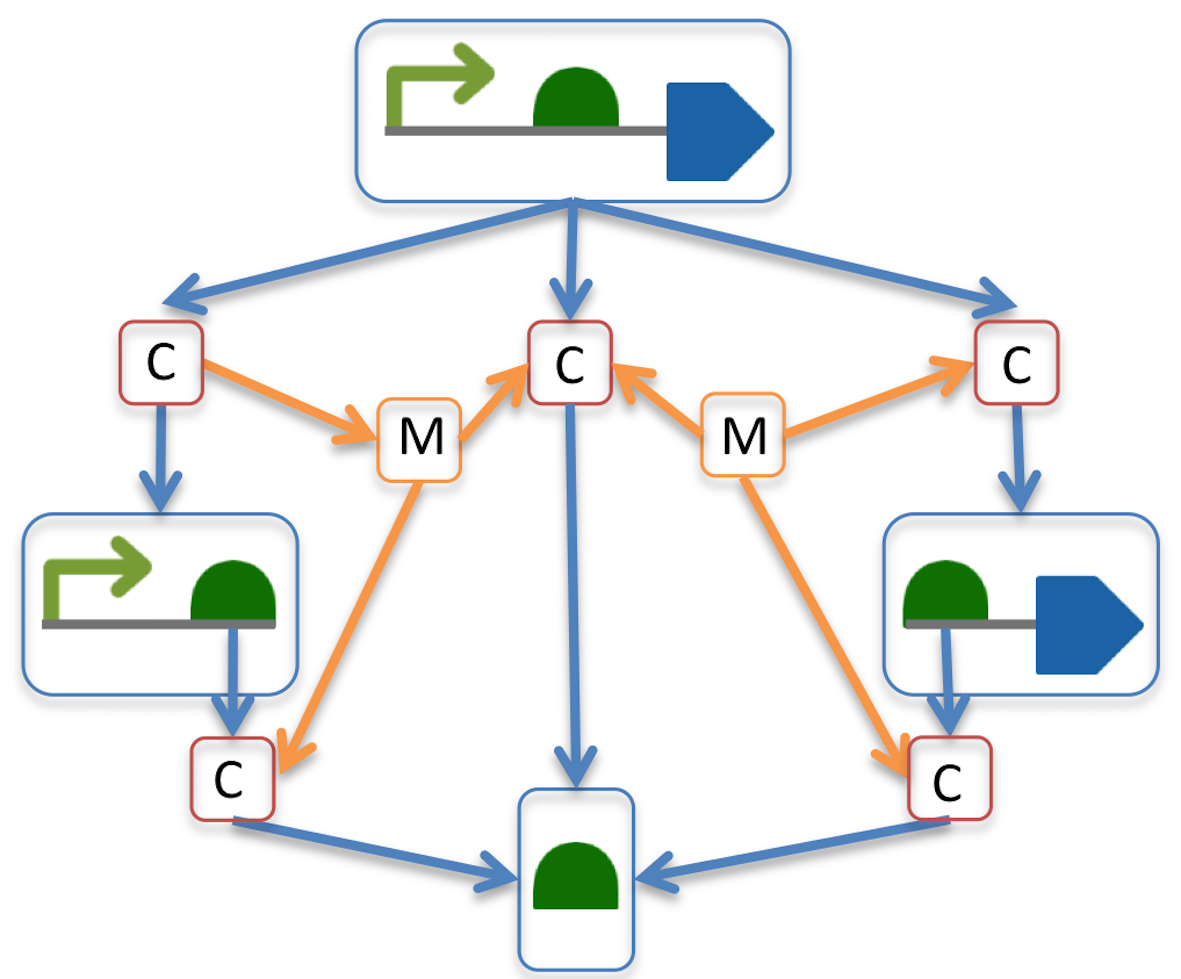
\includegraphics[scale=0.6]{images/MapsTo_Diagram1}
%\caption{Linking Components using MapsTo entities.}
%\label{image:maps_to_diagram1}
%\end{center}
%\end{figure}

\begin{figure}[ht]
\begin{center}
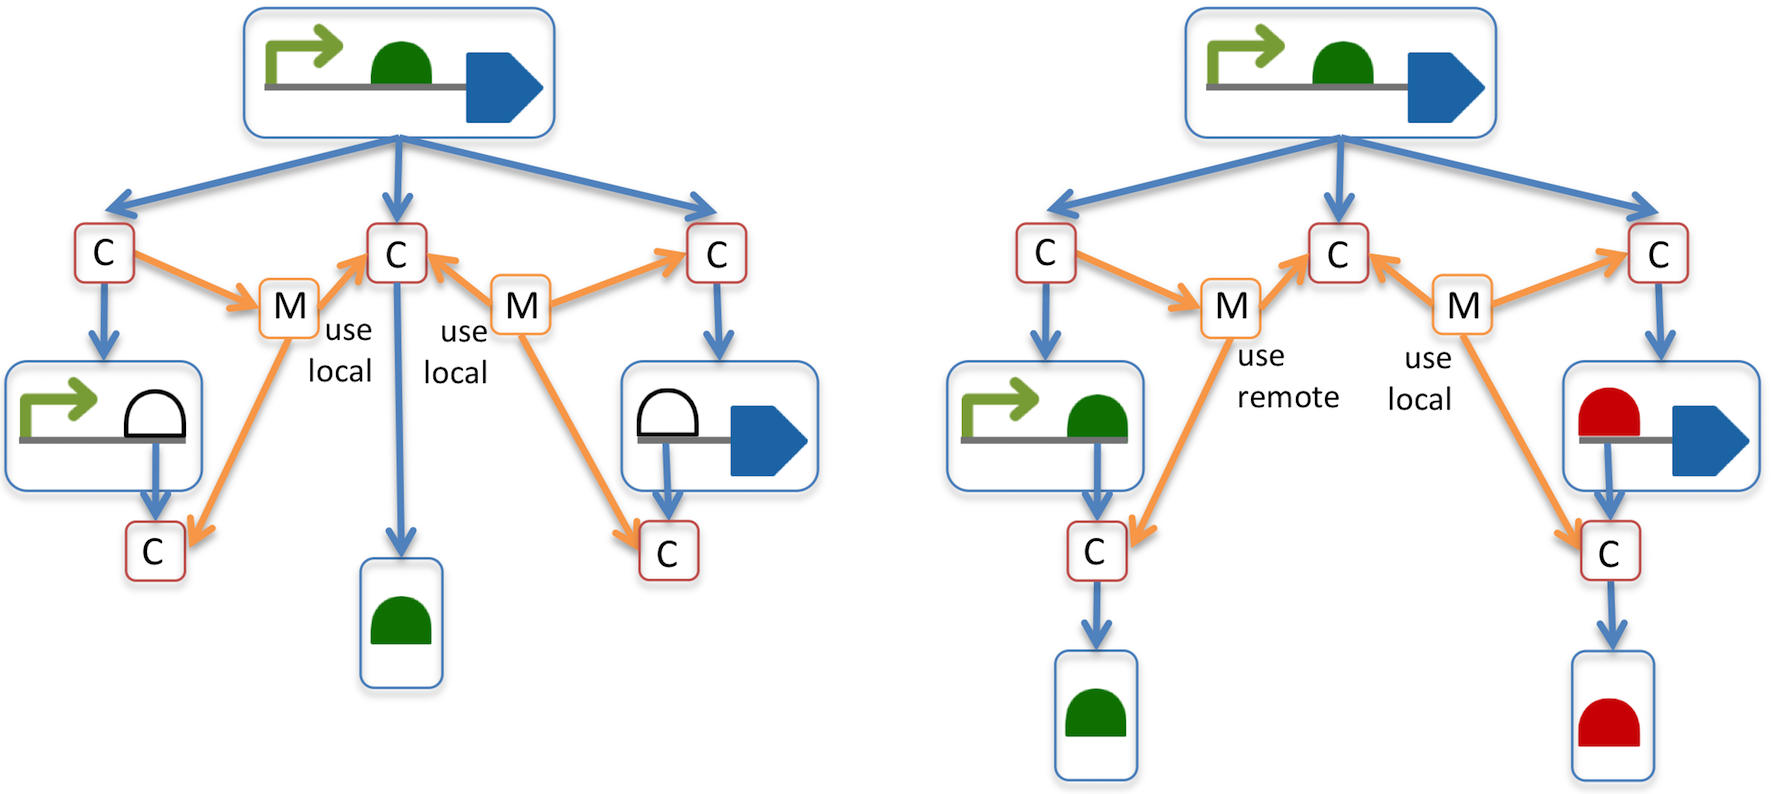
\includegraphics[scale=1]{images/MapsTo_Diagram2}
\caption{Linking Components using MapsTo entities. Boxed with the C label represent Component entities and boxes with the M label represent MapsTo entities.}
\label{image:maps_to_diagram2}
\end{center}
\end{figure}
\Ctodo{Caption: why are some RBSs not filled in?}

An example design of a \sbol{ComponentDefinition} using \sbol{MapsTo} entities is shown at the left hand side of the Figure \ref{image:maps_to_diagram2}. The resulting entity is formed of a promoter, a RBS and a CDS. 
Three sub components to create the design includes: a promoter-RBS \sbol{ComponentDefinition} with a RBS placeholder without detailed definition; a RBS \sbol{ComponentDefinition} with full description; and a RBS-CDS \sbol{ComponentDefinition} with a RBS placeholder, which is also not defined in full detail. 
In the figure, boxes with the C label represent \sbol{Component} entities and boxes with the M label represent the \sbol{MapsTo} entities.
In the design RBSs that are not fully defined are replaced with another RBS \sbol{ComponentDefinition} (displayed in green colour). \sbol{MapsTo} entities attached to sub components for promoter-RBS and RBS-CDS \sbol{ComponentDefinition}s include the ``use local'' refinement to replace RBSs with the fully defined version. In the second design at the right hand side of the figure, \sbol{MapsTo} entities are used to import the RBS from the promoter-RBS \sbol{ComponentDefinition} overwriting the RBS in RBS-CDS \sbol{ComponentDefinition}. 

\Ctodo{Need to expand this explanation a bit more to drive home the points -JB}

\Dtodo{Add a table for refinement values and represent the value when serialized using the rdf:resource property}

\paragraph{Serialization}
The serialization of \sbol{MapsTo} has the following form.
\lstsetsbol
\begin{lstlisting}
<sbol:MapsTo rdf:about="...">
  [\emph{one}] <sbol:refinement>...</sbol:refinement> [\emph{element}]
  [\emph{one}] <sbol:remote rdf:resource="..."/> [\emph{element}]]
  [\emph{one}] <sbol:local rdf:resource="..."/> [\emph{element}]]
</sbol:MapsTo>
\end{lstlisting}

In the example below, a \sbol{FunctionalComponent} entity from the submodule is linked to a \sbol{FunctionalComponent} entity in a parent module. The former is described in the imported \sbol{ModuleDefinition} entity which is referred to by the definition property of the \sbol{Module} entity. The latter is defined in the parent \sbol{ModuleDefinition}, importing the sub module. The full example can be found in \ref{ser:toggleswitch}.
\lstsetsbol
\begin{lstlisting}
<sbol:MapsTo rdf:about="http://sbolstandard.org/example/toggle_switch/submodule/laci_inverter/mapping/Q6QR72">
  <sbol:refinement>USEREMOTE</sbol:refinement>
  <sbol:remote rdf:resource="http://sbolstandard.org/example/toggle_switch/fc/Q6QR72"/>
  <sbol:local rdf:resource="http://sbolstandard.org/example/tetr_inverter/fc/Q6QR72"/>
</sbol:MapsTo>
\end{lstlisting}



\subsubsection{Interaction}
\label{sec:Interaction}

\begin{figure}[ht]
\begin{center}
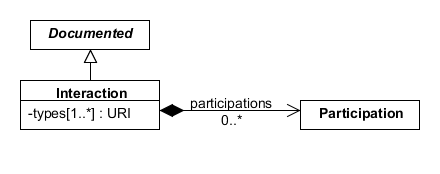
\includegraphics[scale=0.6]{uml/interaction}
\caption[]{Interaction}
\label{uml:interaction}
\end{center}
\end{figure}

\Ctodo{Some of this description is incorrect or unclear}
The Interaction class provides a qualitative basis for asserting the intended function of a given ModuleDefinition object. The proposed data model supports the representation of regulatory interactions, such as activation or repression, and processes from the central dogma of biology, such as transcription and translation. Other supported interaction types include non-covalent binding between a small molecule and TF, and phosphorylation of a TF by an enzyme. 
\Ctodo{What does it mean for an interaction to be supported? --> nothing, pick a better word}

Each Interaction object must specify its type with at least one URI that identifies an appropriate ontology term, such as a term from the Systems Biology Ontology (SBO). If an Interaction object has multiple type URIs, then they must identify synonymous terms. 

\Ctodo{Like the others, SBO is REQUIRED if the term exists, and you can add other stuff.  We also need to explain this up front in the beginning of the section}

Furthermore, each Interaction object must specify its participating \sbol{FunctionalComponent} entities by linking to one or more objects of the Participation class.
\LDtodo{I don't think this is really a MUST}

The serialization of \sbol{Interaction}s has the following form.
\lstsetsbol
\begin{lstlisting}
<sbol:Interaction rdf:about="...">
  [\emph{one or more}] <sbol:type rdf:resource="..."/> [\emph{elements}]
  [\emph{one or more}] <sbol:participation>
                <sbol:Participation rdf:about="...">...</sbol:Participation>
              </sbol:participation> [\emph{elements}]
</sbol:Interaction>
\end{lstlisting}

\Dtodo{Should roles be required types instead?}

\begin{figure}[ht]
\begin{center}
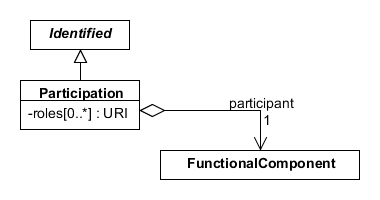
\includegraphics[scale=0.6]{uml/participation}
\caption[]{Participation}
\label{uml:participation}
\end{center}
\end{figure}

\subsubsection{Participation}
\label{sec:Participation}

\Ctodo{Fix the linking and clean grammar}

Each object of the Participation class must specify the role of its participant FunctionalComponent object in its parent Interaction object with at least one URI that identifies an appropriate ontology term. If a Participation object has multiple role URIs, then they must identify synonymous terms. 

\Ctodo{SBO is our REQUIRED term if available, just as in the prior cases}

\Ctodo{Goksel is going to check if there is a superset ontology that should displace SBO}

While the Interaction class provide a qualitative description of genetic function, quantitative descriptions are also needed for genetic design. Instead of introducing a new language for the specification of mathematical models of biology, the proposed data model leverages existing standards and links to them via the Model class. 

\paragraph{Serialization}

The serialization of \sbol{Participation}s has the following form.
\lstsetsbol
\begin{lstlisting}
<sbol:Participation rdf:about="...">
  [\emph{one or more}] <sbol:role rdf:resource="..."/>
  [\emph{one or more}] <sbol:participant rdf:resource="..."/>
</sbol:Participation>
\end{lstlisting}

In the example below, the role of participating \sbol{FunctionalComponent} is defined to be \external{inhibitor}, using the \external{SBO:0000020} term. This component is specified using the participant property of the \sbol{Participation} entity.
\lstsetsbol
\begin{lstlisting}
<sbol:Participation rdf:about="http://sbolstandard.org/example/laci_inverter/interaction/LacI_pLacI/participation/P03023">
  <sbol:role rdf:resource="http://identifiers.org/biomodels.sbo/SBO:0000020"/>
  <sbol:participant rdf:resource="http://sbolstandard.org/example/laci_inverter/fc/P03023"/>
</sbol:Participation>
\end{lstlisting}

\subsection {Collection}
\label{sec:Collection}
The \sbol{Collection} class is a class that groups together a set of \sbol{TopLevel} objects that have something in common. 
Some examples of \sbol{Collection} objects:
\begin{itemize}
\item Results of a query to find all \sbol{ComponentDefinition} objects that function as promoters in a repository.
\item A set of \sbol{ModuleDefinition} objects representing a library of NAND gates.
\item A \sbol{ModuleDefinition} for a complex design, and all of the \sbol{ModuleDefinition}, \sbol{ComponentDefinition}, \sbol{Sequence}, and \sbol{Model} objects used to provide its full specification.
\end{itemize}

\begin{figure}[ht]
\begin{center}
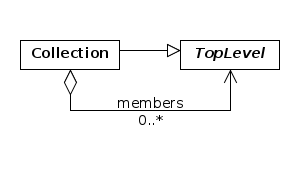
\includegraphics[scale=0.6]{uml/collection}
\caption[]{The Collection class}
\label{uml:collection}
\end{center}
\end{figure}

\subsubsection*{The member property}
The member property has a data type of URI and has the \sbol{identity} value of a \sbol{TopLevel} entity.  A collection may have any number of members, including none.

\subsubsection*{Serialization}

The serialization of \sbol{Collection} objects has the following form:

\lstsetsbol
\begin{lstlisting}
<sbol:Collection rdf:about="...">
              ...
  [\emph{one or more}] <sbol:member rdf:resource="..."/> [\emph{element}]
</sbol:Collection>
\end{lstlisting}

\Ctodo{We should make all of the example URIs compliant}

The example below shows the serialization of a \sbol{Collection} object grouping together a library of constitutive promoters.
\lstsetsbol
\begin{lstlisting}
<?xml version="1.0" ?>
<rdf:RDF xmlns:rdf="http://www.w3.org/1999/02/22-rdf-syntax-ns#" xmlns:dcterms="http://purl.org/dc/terms/" xmlns:sbol="http://sbols.org/v2#">
  <sbol:Collection rdf:about="http://parts.igem.org/Promoters/Catalog/Anderson">
    <sbol:displayId>Anderson</sbol:displayId>
    <dcterms:title>Anderson promoters</dcterms:title>
    <dcterms:description> The Anderson promoter collection</dcterms:description>
    <sbol:member rdf:resource="http://parts.igem.org/wiki/index.php/Part:BBa_J23119"/>
    ...
    <sbol:member rdf:resource="http://parts.igem.org/wiki/index.php/Part:BBa_J23118"/>
  </sbol:Collection>
</rdf:RDF>

\end{lstlisting}
\label{ser:Collection}




\subsection{Extending the SBOL Representation:  Annotations}
\label{sec:annotations}

SBOL does not attempt to represent all information about a biological system, since many things do not yet have a clear ``right way'' to be represented, such as design intent, biological context, or performance data.
Instead, SBOL allows the embedding of application specific data that are not captured by the SBOL standard. 
Such data are optional, but can be computationally generated and exchanged via SBOL documents without getting lost. 

To do this, SBOL provides an ``annotation'' mechanism for attaching arbitrary information to SBOL objects, which allows SBOL models to be connected with any other models in an extensible manner.
In particular, three models are supported for connecting the SBOL model with other, possibly application-specific models:
\begin{itemize}
\item Information that is ``part'' of an SBOL object (i.e., a ``filled diamond'' relationship) is annotated simply by adding non-conflicting properties and custom identity entries to an SBOL object.  An example might be source information about the registry from which a \sbol{ComponentDefinition} was imported.
\item Information that is an independent object is annotated by wrapping it inside of a \sbol{GenericTopLevel} object.  An example might be a data sheet describing the performance of a \sbol{ModuleDefinition} in some particular context.
\item Conversely, rather than embedding external objects in SBOL, SBOL objects can also be linked from or embedded inside of other data models.  The only requirement is that some URI resolution mechanism must be available that allows the links between SBOL objects thus separated from one another to be followed when needed.
\end{itemize}

\Ctodo{Make sure we explain about annotations up in the motivation and overview, since it's really, really important.}

\subsubsection{Annotating SBOL objects}

\LDtodo{URI: plain or courier?}

Each \sbol{Identified} object may have a number of annotations in the form of name/value property pairs. 
Property names are specified by qualified names as \external{URI}s, each formed of a namespace and a local name. 
Values can be \external{URI}s or \external{Literal} data (for example, \external{String}, \external{Integer}, \external{Double}, \external{Boolean}) or custom \sbol{Identified} entities initialized with application specific types. 
These custom \sbol{Identified} entities can further be annotated with the scheme described here. These custom entities are either serialized within an SBOL entity being annotated, or referenced using an \external{URI} annotation and embedded within the the annotated entity's parent.
\Dtodo{Make sure if we have a choice here!}

\begin{figure}[!ht]
\begin{center}
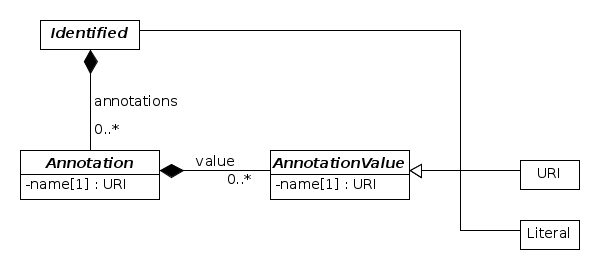
\includegraphics[scale=0.6]{uml/identified_annotations}
\caption[]{Annotating SBOL's Identified entities with application specific data.}
\label{uml:identified_annotations}
\end{center}
\end{figure}
\Dtodo{I think this should actually be: add any object here of your own custom class (which MUST NOT use the SBOL namespace), not ``make chains of identified''}
\Dtodo{Is this figure how the annotations are actually handled in libSBOLj?}
\Dtodo{Consider putting Identified, uRI, and Literal on the bottom so that inheritance arrows point in the same direction as they do in other diagrams. Another consideration for maintaing consistency with the other diagrams is to add arrow heads to the opposite ends of the black diamond relations. - Nic}

Each annotation is serialised as an RDF subject-property-object triplet in which the subject is the SBOL object being annotated, the property is the annotation name, and the object is the annotation value. Simple values URIs are serialised as RDF literals, and URI values are represented with the \external{\path{http://www.w3.org/1999/02/22-rdf-syntax-ns#resource}} RDF property. If the annotation value is another complex object then the object is embedded as an RDF resource, which can further be annotated similarly.
\Dtodo{If we allow URI reference of a custom object stored, then update this paragraph}

\paragraph{Serialization}
The ComponentDefinition example for a promoter serialized below shows how annotations can be added to SBOL objects. Annotations are added using the relevant information from the Parts Registry. Annotation property names are qualified with the \external{http://www.partsregistry.org/} namespace, which is prefixed using \external{pr}. The first annotation is named as \external{pr:group}, indicating the iGEM group designing the promoter, and has a \external{String} value. The second \external{pr:experience} annotation has a \external{URI} value and is serialised as an RDF resource pointing to the information Web page on the Parts Registry for the promoter. The  \external{pr:information} property represents a complex annotation which is a type of \external{pr:Information} and includes information about the regulatory details of the promoter using Parts Registry categories.   

\begin{figure} [ht]
\lstsetsbol
\begin{lstlisting}
<?xml version="1.0" ?>
<rdf:RDF xmlns:pr="http://www.partsregistry.org/" xmlns:rdf="http://www.w3.org/1999/02/22-rdf-syntax-ns#" xmlns:dcterms="http://purl.org/dc/terms/" xmlns:sbol="http://sbols.org/v2#">
  <sbol:ComponentDefinition rdf:about="http://www.partsregistry.org/Part:BBa_J23119">
    <pr:group>iGEM2006_Berkeley</pr:group>
    <pr:experience rdf:resource="http://www.partsregistry.org/Part:BBa_J23119:Experience"/>
    <pr:information>
      <pr:Information rdf:about="http://parts.igem.org/cgi/partsdb/part_info.cgi?part_name=BBa_J23119">
        <pr:sigmafactor>//rnap/prokaryote/ecoli/sigma70</pr:sigmafactor>
        <pr:regulation>//regulation/constitutive</pr:regulation>
      </pr:Information>
    </pr:information>
    <dcterms:title>J23119</dcterms:title>
    <dcterms:description>Constitutive promoter</dcterms:description>
    <sbol:type rdf:resource="http://www.biopax.org/release/biopax-level3.owl#DnaRegion"/>
    <sbol:role rdf:resource="http://purl.org/obo/owl/SO#SO_0000167"/>
  </sbol:ComponentDefinition>
</rdf:RDF>
\end{lstlisting}
\label{ser:Annotation}
\end{figure}




\subsubsection{GenericTopLevel}  
\label{sec:GenericTopLevel}
SBOL documents can also be annotated at the top level. 
SBOL's \sbol{GenericTopLevel} is a top-level entity whose only purpose is to include a set of annotations as described above. 
Entities that have independent existence (i.e., would be another ``top level'' class) and are not recognised by the SBOL standard are loaded into these top level entities. 
These \sbol{GenericTopLevel} entities can thus be safely used by tools to exchange non-SBOL data embedded separately within SBOL.
As with any other top level entities, \sbol{GenericTopLevel} entities may include SBOL properties such as \sbol{name}, \sbol{description}, \sbol{displayId} and so on. The type of data found in the generic entity is indicated using the standard \external{rdf:type} property.

\Ctodo{rdf:type should be rdfType}

\begin{figure}[ht]
\begin{center}
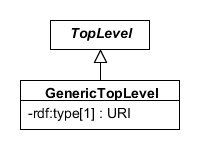
\includegraphics[scale=0.6]{uml/generictoplevel}
\caption[]{Annotating SBOL documents with GenericTopLevel entities.}
\label{uml:generictoplevel}
\end{center}
\end{figure}

The example below shows how a datasheet object can be added to an SBOL document using the \sbol{GenericTopLevel} class. 
The J23119 promoter example is annotated with the URI of a top Level Datasheet object, here defining the annotation properties using the custom \external{\path{http://www.myapp.org/}} namespace and the \external{myapp} prefix. 
The datasheet object, with the data type of \external{myapp:Datasheet}, is accessed using the \external{URI} value specified by the \external{myapp:characterizationData} property of the promoter component definition. 
The datasheet object is further annotated with the transcription rate and the URI for the actual characterization data using the \external{myapp:transcriptionRate} and \external{myapp:characterizationData} properties respectively.
Finally, this data sheet is linked from the component is describes using an annotation with a \external{myapp:datasheet} property whose value is the data sheet's URI.

\begin{figure}[ht]
\lstsetsbol
\begin{lstlisting}
<?xml version="1.0" ?>
<rdf:RDF xmlns:myapp="http://www.myapp.org/" xmlns:rdf="http://www.w3.org/1999/02/22-rdf-syntax-ns#" xmlns:dcterms="http://purl.org/dc/terms/" xmlns:sbol="http://sbols.org/v2#">
  <sbol:ComponentDefinition rdf:about="http://www.partsregistry.org/Part:BBa_J23119">
    <myapp:datasheet rdf:resource="http://www.myapp.org/datasheet/1"/>
    <dcterms:title>J23119</dcterms:title>
    <dcterms:description>Constitutive promoter</dcterms:description>
    <sbol:type rdf:resource="http://www.biopax.org/release/biopax-level3.owl#DnaRegion"/>
    <sbol:role rdf:resource="http://purl.org/obo/owl/SO#SO_0000167"/>
  </sbol:ComponentDefinition>
  <myapp:Datasheet rdf:about="http://www.myapp.org/datasheet/1">
    <myapp:characterizationData rdf:resource="http://www.myapp.org/measurement/1"/>
    <myapp:transcriptionRate>1</myapp:transcriptionRate>
    <dcterms:title>Datasheet 1</dcterms:title>
  </myapp:Datasheet>
</rdf:RDF>

\end{lstlisting}
\label{ser:GenericTopLevel}
\end{figure}